\documentclass[a4paper, 12pt]{book}

% General Settings
\usepackage[paper = a4paper, margin = 1in]{geometry}
\usepackage[italian]{babel}
\usepackage[utf8]{inputenc}
\usepackage[T1]{fontenc}
\usepackage{hyperref}
\usepackage{graphicx}
\usepackage[small]{caption}
\usepackage{subfig}
\usepackage[usenames,dvipsnames]{xcolor}
\usepackage{graphicx,color,listings}
\usepackage{float}
\usepackage{booktabs}
\usepackage{hologo}
\usepackage{colortbl}

% Math and physic packages
\usepackage{amsmath,amssymb,amsthm}
\usepackage{mathrsfs}
\usepackage{mathdots}
\usepackage{mathtools}
\usepackage{physics}
\numberwithin{equation}{section}
\numberwithin{figure}{chapter}


% New or renewed commands
\newcommand{\lecture}[2]{{\scshape{Lezione #1 - #2}} \par}
\newtheorem{definizione}{Definizione}[chapter]
\newtheorem{teorema}{Teorema}[chapter]
\newtheorem{esempio}{Esempio}[chapter]
\renewcommand{\thefootnote}{\roman{footnote}}

% Documents
\begin{document}
    \begin{titlepage}
        \begin{center}
            \vspace*{5cm}
            {\scshape\LARGE Università degli Studi di Milano - Bicocca \par}
            \vspace{1.0cm}
            \line(1,0){400} \\
            {\huge\bfseries Tecnologie quantistiche applicate \par}
            \line(1,0){400} \\
 	        \vspace{0.5cm}
            {\Large Raccolta di appunti, dispense e libri \par}
            \vspace{1.0cm}
            {Anno accademico 2021/2022 \par}
            \vspace{0.5cm}
            {\bfseries Marco Gobbo\par}
            \vspace{0.5cm}
            {\url{https://github.com/marcogobbo/tecnologie-quantistiche} \par}
            \vspace*{\fill}
            {\large \today \par}
        \end{center}
    \end{titlepage}
    \tableofcontents
    %%%%%%%%%%%%%
% LECTURE 1 %
%%%%%%%%%%%%%

\chapter{Meccanica quantistica}

\lecture{1}{07/10/2021}
\section{Stati e qubit}
Prima di addentrarci nello studio delle tecnologie quantistiche, risulta opportuno fare alcuni richiami di meccanica quantistica implementando alcuni concetti che ci saranno poi utili in futuro. In particolare iniziamo velocemente ricordando il primo postulato della meccanica quantistica
\begin{itemize}
    \item \textbf{I Postulato} (\textbf{Stato}): Che cos'è uno stato? Utilizziamo la notazione di Dirac per rappresentare un vettore $\ket{\psi}$ di uno spazio di Hilbert $\mathcal{H}$ (molto spesso uno spazio vettoriale finito dimensionale) e diremo che $\ket{\psi} \in \mathcal{H}$. Uno stato è un \textbf{raggio} tale che $\norm{\ket{\psi}} = 1$ (per la conservazione della probabilità) e $\ket{\psi} \cong e^{i \alpha} \ket{\psi}$ \footnote{La notazione $\cong$ significa "equivalente a".} con $\alpha \in \mathbb{R}$. Dato che la fase globale è irrilevante, quando due stati differiscono per una fase hanno il medesimo effetto fisico. 
\end{itemize}
Procediamo ora con il definire cosa sia un qubit
\begin{definizione}[\textbf{Qubit}]
    Un qubit è un qualsiasi sistema a due livelli. Ogni sistema quantomeccanico può essere un qubit, ad esempio si può creare utilizzando le due differenti polarizzazioni del fotone, utilizzando l’allineamento dello spin di un nucleo immerso in un campo magnetico uniforme, utilizzando la tecnica della trappola ionica, sistemi superconduttivi, \dots
\end{definizione}
\noindent Davide di Vincenzo, nel 2000, ha indicato cinque criteri necessari per la scelta di un sistema fisico adatto per la computazione quantistica:
\begin{enumerate}
    \item Un sistema fisico scalabile con qubit ben caratterizzati;
    \item La capacità di inizializzare lo stato dei qubit a un semplice stato fiduciale;
    \item Tempi di decoerenza lunghi e rilevanti;
    \item Un insieme "universale" di porte quantistiche;
    \item Una capacità di misurazione specifica per qubit.
\end{enumerate}
La meccanica quantistica si occupa di descrivere il comportamento del nostro sistema a due livelli mediante una hamiltoniana. Per fare ciò lavoriamo in spazi di Hilbert bidimensionali $\mathcal{H}=\mathbb{C}^2$, quindi le hamiltoniane di questi sistemi sono degli operatori definiti su $\mathbb{C}^2 \rightarrow \mathbb{C}^2$. Gli stati in cui si trova il nostro sistema sono descritti da funzioni d'onda generiche $\psi \in \mathbb{C}^2$, in particolar modo possono essere decomposte sulla base computazionale $\{\ket 0, \ket 1\}$. Avremo quindi che 
\begin{equation*}
    \begin{array}{l}
        \hat H \ket 0 = E_0 \ket 0 \\
        \hat H \ket 1 = E_1 \ket 1 \, ,
    \end{array}
\end{equation*}
dove
\begin{equation*}
    \begin{array}{l}
        \ip{0}{0}=\ip{1}{1}=1 \\
        \ip{0}{1}=\ip{1}{0}=0 \, .
    \end{array}
\end{equation*}
Per cui ogni stato generico $\ket \psi$ può essere scritto come combinazione lineare di $\{\ket 0, \ket 1\}$
\begin{equation*}
    \ket \psi = a \ket 0 + b \ket 1 \, ,
\end{equation*}
con $a,b \in \mathbb{C}$ e soddisfacenti la condizione di conservazione di probabilità
\begin{equation*}
    \abs{a}^2+\abs{b}^2=1 \, .
\end{equation*}
Osserviamo che, per come è definito, $\ket \psi$ è uno \textbf{stato puro}, ci dà la massima conoscenza che possiamo ottenere da questo sistema. Infatti abbiamo una probabilità pari a $\abs{a}^2$ di ottenere $\ket 0$ e una probabilità pari a $\abs{b}^2$ di ottenere $\ket 1$. Dobbiamo misurare un numero infinito di volte per poter ottenere queste distribuzioni di probabilità, tuttavia non possiamo eseguire una misura successiva per estrarre ulteriori informazioni sul nostro stato $\ket \psi$ poiché quest'ultimo sarà collassato in $\ket 0$ oppure $\ket 1$. Per determinare univocamente $\alpha$ e $\beta$ si necessiterebbe un'infinità di esperimenti su un'infinità di stati tutti preparati nel medesimo stato $\ket \psi$. La massima conoscenza che possiamo estrarre non è molta, questo fatto è stato oggetto di discussione per molti anni. In particolar modo ci si è chiesti se la teoria meccanica quantistica fosse una teoria completa o meno\footnote{Einstein, A., Podolsky, B., \& Rosen, N. (1935). Can Quantum-Mechanical Description of Physical Reality Be Considered Complete?. Phys. Rev., 47, 777–780.}.\\
Come abbiamo già accennato, $a$ e $b$ sono coefficienti complessi, attraverso la notazione esponenziale possiamo scriverli come
\begin{equation*}
    a=\abs{a}e^{i\theta_0} \qquad b=\abs{b}e^{i\theta_1}\, ,
\end{equation*}
in questo modo
\begin{equation*}
    \begin{aligned}
        \ket \psi &= \abs{a}e^{i\theta_0}\ket 0 + \abs{b}e^{i\theta_1}\ket 1 \\
                  &= \underbrace{e^{i\theta_0}}_{\mathclap{\text{Fase globale}}}\Big(\abs{a}\ket 0 + \abs{b}\underbrace{e^{i\left(\theta_1-\theta_0\right)}}_{\mathclap{\text{Fase relativa}}}\ket 1\Big) \, .
    \end{aligned}
\end{equation*}
Quando misuriamo uno stato, la \textit{fase globale} risulta essere irrilevante, ciò che conta è la \textit{fase relativa} perché può dar luogo a fenomeni come l'interferenza.
\begin{esempio}[Fase relativa]
    Consideriamo gli stati $\ket 0 e \ket 1$, per scrivere i seguenti stati
    \begin{equation*}
        \ket{\psi_1}=\frac{\ket 0 + \ket 1}{\sqrt 2}\, \qquad \ket{\psi_2}=\frac{\ket 0 - \ket 1}{\sqrt 2} 
    \end{equation*}
    In questo caso il segno meno proviene dalla fase relativa. $\ket{\psi_1}$ e $\ket{\psi_2}$ forniscono lo stesso risultato per una misura di energia (lo si può verificare calcolando $\mel{\psi_i}{\hat H}{\psi_i}$), tuttavia riusciamo a distinguerli se facciamo una misura diversa. Ad esempio possiamo considerare la matrice di Pauli
    \begin{equation*}
        \sigma_x = \begin{pmatrix}
                    0 & 1 \\
                    1 & 0
                   \end{pmatrix}\, ,
    \end{equation*}
    $\ket{\psi_1}$ e $\ket{\psi_2}$ sono autostati di $\sigma_x$ con autovalori, rispettivamente, $1$ e $-1$.
\end{esempio}
\noindent Uno dei problemi principali nell'aver a che fare con sistemi quantistici è trovare l'evoluto temporale di un certo stato, perché abbiamo delle hamiltoniane che descrivono ad esempio il rumore degli strumenti, la temperatura dell'ambiente, \dots L'equazione di Schrödinger si comporta bene nel descrivere l'evoluzione di \textbf{sistemi chiusi}, ma un qubit è, in generale, un \textbf{sistema aperto} che si lega a sistemi esterni e quindi la conoscenza sul suo stato tende a diminuire, finché non perdiamo completamente l'informazione che possedeva all'inizio. Questo fatto è legato al \textbf{tempo di coerenza}. Ci sono vari modi per tenere conto di queste interazioni così da poter descrivere al meglio il nostro sistema a due livelli.\\
Supponiamo di avere un sistema chiuso che evolve secondo l'equazione di Schrödinger
\begin{equation*}
    \hat H \ket{\psi(t)}=i\hbar \partialderivative{t}\ket{\psi(t)}\, ,
\end{equation*}
dove $\ket{\psi(t)}=\hat U(t)\ket{\psi(0)}$. $\hat U$ in questo caso è un operatore unitario che può essere espresso, se l'hamiltoniana è costante nel tempo, come
\begin{equation*}
    \hat U(t)=e^{-\frac{i}{\hbar}\hat H t}\, .
\end{equation*}
Pertanto, considerando gli autostati dell'hamiltoniana 
\begin{equation*}
    \hat H \ket{i}=E_i\ket{i}\, ,
\end{equation*}
e riscrivendo il nostro stato iniziale in termini di autostati dell'hamiltoniana
\begin{equation*}
    \ket{\psi(0)}=\sum_i a_i\ket i\, ,
\end{equation*}
possiamo valutare il nostro stato al tempo generico $t$ come
\begin{equation*}
    \ket{\psi(t)}=\sum_i a_ie^{-\frac i \hbar \hat H t}\ket i=\sum_i a_i e^{-\frac i \hbar E_i t}\ket i \qquad \text{dove} \quad a_i(t)=a_i(0)e^{-\frac i \hbar E_i t}\, .
\end{equation*}
Da questo caso generale possiamo trattare il nostro sistema a due livelli, in questo caso l'hamiltoniana sarà
\begin{equation*}
    \hat H = \begin{pmatrix}
        E_0 & 0 \\
        0 & E_1
       \end{pmatrix}\, ,
\end{equation*}
applicando l'equazione di Schrödinger sui coefficienti
\begin{equation*}
    i\hbar\derivative{a_0(t)}{t}=E_0a_0(t)\, ,
\end{equation*}
\begin{equation*}
    i\hbar\derivative{a_1(t)}{t}=E_1a_1(t)\, ,
\end{equation*}
troviamo che il nostro stato finale al tempo generico $t$ sarà
\begin{equation*}
    \ket{\psi(t)}=\underbrace{e^{-\frac{i}{\hbar}E_0t}}_{\text{Fase globale}}\Big(a_0(0)\ket 0 +\underbrace{e^{-\frac{i}{\hbar}(E_1-E_0)t}a_1(0)}_{\text{Fase relativa}}\ket 1\Big)\, .
\end{equation*}
Ancora una volta, la fase globale non produce alcun effetto, ciò che notiamo è che l'evoluzione temporale cambia la fase relativa tra gli stati $\ket 0$ e $\ket 1$. Questo spiega perché se abbiamo una interazione che disturba il nostro sistema possiamo avere un cambio nella fase relativa, questo è dato dal fatto che abbiamo una variazione in termini energetici. Questo disturbo è generato da tutto ciò che è esterno al sistema a due livelli. Se perdiamo il controllo su questa fase, perdiamo tutta l'informazione che abbiamo su $\ket{\psi(t)}$, e se questo accade, non abbiamo più uno stato puro. Per questo motivo necessitiamo qualcosa che vada oltre al concetto di funzione d'onda generica $\psi$.

\section{Matrice densità}
Vogliamo realizzare uno stato puro $\ket \psi$ che sia una combinazione pura di stati $\ket 0$ e $\ket 1$:
\begin{equation*}
    \ket \psi = a\ket 0 + b \ket 1\, ,
\end{equation*}
nella realtà quando cerchiamo di realizzare questo stato, abbiamo un'indeterminazione classica rappresentata da una distribuzione di probabilità di ottenere lo stato esatto oppure uno stato simile. Supponiamo di avere un insieme di stati che indichiamo con $\{p_i, \ket{\psi_i}\}$, dove $p_i$ è la probabilità classica di ottenere un generico stato. Questi stati $\ket{\psi_i}$ sono tutti stati puri, ma non sappiamo quale sia quello giusto e la sua conoscenza è persa. Tutte queste informazioni sono contenute nella \textbf{matrice densità} che rappresenta una distribuzione classica di probabilità.\\
Dal punto di vista della teoria della meccanica quantistica, esiste un altro modo per introdurre la teoria anziché sfruttare gli stati $\psi$. Quello che si fa è sfruttare la matrice densità che è un operatore che agisce nel seguente modo
\begin{equation*}
    \hat \rho \ket{\psi_i}=p_i\ket{\psi_i}\, ,
\end{equation*}
dove $p_i$ rappresenta la probabilità di ottenere lo stato i-esimo. La matrice densità è ora una miscela di stati puri
\begin{equation*}
    \hat \rho = \sum_i p_i \op{\psi_i}{\psi_i}
\end{equation*}
e descrive la mancanza di conoscenza sui sistemi quantistici che avevamo precedentemente. Se utilizzassimo lo stesso operatore $\hat U$ per descrivere l'evoluto temporale di $\ket{\psi_i} \overset{t}{\longrightarrow} \hat U\ket{\psi_i}$, come possiamo applicarlo a $\hat \rho$?
\begin{equation*}
    \hat \rho = \sum_i p_i \op{\psi_i}{\psi_i} \longrightarrow \sum_i p_i \hat U\op{\psi_i}{\psi_i}\hat U^\dagger \,
\end{equation*}
\begin{equation*}
    \hat U \hat \rho \hat U^\dagger = \hat \rho ' \, .
\end{equation*}
Vediamo se le distribuzioni di probabilità classiche, nel caso di stati ortonormali, vengono conservate:
\begin{proof}\mbox{}\\*
    \noindent A $t=0$ :
    \begin{equation*}
          \hat \rho \ket{\psi_i (0)} = p_i \ket{\psi_i (0)} \\
    \end{equation*}
    A $t>0$ :
    \begin{equation*}
        \begin{aligned}
            \hat \rho' \ket{\psi_i (t)} &= \hat U \hat \rho \hat U^\dagger \hat U \ket{\psi_i (0)} \\      
                                        &=\hat U \hat \rho \ket{\psi_i (0)} \\
                                        &=\hat U p_i \ket{\psi_i (0)} \\
                                        &=p_i U \ket{\psi_i (0)} \\
                                        &=p_i\ket{\psi_i (t)}
        \end{aligned}
    \end{equation*}

    \noindent La probabilità $p_i$ non è cambiata nel tempo, ma lo stato sì perché ora è $\ket{\psi_i (t)}$ che non è uguale a $\ket{\psi_i (0)}$.
\end{proof}
    %%%%%%%%%%%%%
% LECTURE 2 %
%%%%%%%%%%%%%
\newpage
\noindent \lecture{2}{08/10/2021}

\section{Osservabili}\label{sec:osservabili}

\begin{itemize}
    \item \textbf{II Postulato} (\textbf{Osservabili}): Che cosa si può misurare in QM? Vengono misurate le \textbf{osservabili}, ossia \textbf{operatori autoaggiunti} (o \textbf{hermitiani}) $\hat{A}$ tali che
    \begin{equation*}
        \hat{A}: \mathcal{H}\rightarrow \mathcal{H} \, \text{ con } \, \hat{A}^\dagger = \hat{A} \, ,
    \end{equation*}
    dove più precisamente $\hat{A}^\dagger \equiv (\hat{A}^t)^\ast$. Dal punto di vista degli elementi di matrice, calcolare l'aggiunto di $A_{ij}$ significa $A^\dagger_{ij} = A^\ast_{ji}$. Dunque le matrici autoaggiunte (hermitiane) sono tali che $A^\dagger \equiv (A^t)^\ast = A$.  
\end{itemize}

\noindent In base a ciò che abbiamo visto sulla notazione braket  ($\bra{\phi} = \ket{\phi}^\dagger$) abbiamo necessariamente che

\begin{equation*}
    \ket{\psi} = B \ket{\phi} \, , \quad \Rightarrow \quad  \bra{\psi} = \bra{\phi} B^\dagger \, .
\end{equation*}

\noindent Focalizzando la nostra attenzione sugli operatori autoaggiunti, richiamiamo un importante teorema di algebra lineare:
\begin{teorema}[\textbf{Teorema Spettrale}]
    Sia $\hat{A}$ un operatore autoaggiunto su uno spazio di Hilbert $\mathcal{H}$. Allora esiste una base ortonormale di $\mathcal{H}$ composta da autovettori di $\hat{A}$, ossia $\exists$ $\lbrace \ket{n} \rbrace \in \mathcal{H}$ tale che $\hat{A} \ket{n} = a_n \ket{n}$ dove gli autovalori $a_n \in \mathbb{R}$.
\end{teorema}

\noindent Si noti dal teorema che $\braket{n}{m} = \delta_{nm}$ dove $n,m = 1, \ldots, N$ con $N \equiv \dim \mathcal{H}$. Trattandosi di una base, qualsiasi vettore dello spazio di Hilbert può essere scritto come combinazione lineare di tali vettori: 

\begin{equation*}
    \ket{\psi} = \sum_{n=1}^N \alpha_n \ket n \, , \, \text{ dove } \, \alpha_n \equiv \braket{n}{\psi} \in \mathbb{C} \, .
\end{equation*}

\noindent Ritornando al nostro caso del sistema a due livelli, lo spazio di Hilbert in esame è $\mathbb{C}^2$, dove consideriamo la \textbf{base canonica} (o \textbf{base computazionale}) data dagli stati $\ket 0$ e $\ket 1$ (si vedano le definizioni in \eqref{computational_basis}). In questo spazio vettoriale gli operatori sono rappresentati da matrici $2 \times 2$. La più generale matrice $2 \times 2$ hermitiana contenente 4 parametri reali è

\begin{equation*}
    A = 
    \begin{pmatrix}
        a+b & c-id \\ 
        c+id & a-b
    \end{pmatrix} \, ,
\end{equation*}

\noindent dove $a, b, c, d \in \mathbb{R}$. Si noti che sulla diagonale le entrate sono puramente reali. Così come abbiamo decomposto uno stato generico $\ket{\psi}$ mediante combinazione lineare di autovettori $\ket{n}$, possiamo decomporre il generico operatore hermitiano di $\mathbb{C}^2$ come 

\begin{equation}\label{generical_matrix_C2}
    A = a \mathbb{I} + c \sigma_1 + d \sigma_2 + b \sigma_3 \, ,
\end{equation}

\noindent dove $\mathbb{I}$ è la matrice \textbf{identità} e $\sigma_1, \sigma_2, \sigma_3$ sono le \textbf{matrici Pauli}:

\begin{equation}\label{Pauli_matrices}
    \sigma_1=
    \begin{pmatrix}
        0 & 1 \\
        1 & 0
    \end{pmatrix} \, , \ \ \ \ \
    \sigma_2=
    \begin{pmatrix}
        0 & -i \\
        i & 0
    \end{pmatrix} \, , \ \ \ \ \
    \sigma_3=
    \begin{pmatrix}
        1 & 0 \\
        0 & -1
    \end{pmatrix} \, . \ \ \ \ \
\end{equation}

\noindent Si ricordi che le matrici di Pauli sono i generatori del momento angolare in QM e sono infatti utilizzate per descrivere l'operatore di spin $\hat{\vec{S}} = \frac{\hbar}{2} \hat{\vec{\sigma}}$. I relativi autovalori e autovettori sono mostrati nella Tabella \ref{tab:Pauli_eig}.

\begin{table}[!ht]
	\centering
    \begin{tabular}{ccc}
        \toprule
        \textbf{Matrice di Pauli} & \textbf{Autovettori} & \textbf{Autovalori}  \\
        \midrule
        $\sigma_1$ & $\ket + = \frac{1}{\sqrt 2} \begin{pmatrix} 1 \\ 1 \end{pmatrix}, \qquad \ket - = \frac{1}{\sqrt 2} \begin{pmatrix} 1 \\ -1 \end{pmatrix} $ & $\lbrace 1, -1 \rbrace$ \\
        $\sigma_2$ & $\ket i = \frac{1}{\sqrt 2} \begin{pmatrix} 1 \\ i \end{pmatrix}, \qquad \ket{-i} = \frac{1}{\sqrt 2} \begin{pmatrix} 1 \\ -i \end{pmatrix} $ & $\lbrace 1, -1 \rbrace$ \\
        $\sigma_3$ & $\ket 0 = \begin{pmatrix} 1 \\ 0 \end{pmatrix}, \qquad \ket 1 = \begin{pmatrix} 0 \\ 1 \end{pmatrix} $ & $\lbrace 1,-1 \rbrace$ \\
        \bottomrule
    \end{tabular}\\
    \caption{Autovettori e autovalori delle matrici di Pauli.}
    \label{tab:Pauli_eig}
\end{table}

\noindent Dato che in futuro ci tornerà utile, osserviamo che gli autovettori di $\sigma_1$ e $\sigma_2$ possono essere espressi mediante base computazionale come

\begin{equation}\label{basi_di_sigma_12}
    \ket + = \frac{\ket 0 + \ket 1}{\sqrt 2} \, , \quad \ket - = \frac{\ket 0 - \ket 1}{\sqrt 2} \, , \quad \ket i = \frac{\ket 0 + i \ket 1}{\sqrt 2} \, , \quad \ket{-i} = \frac{\ket 0 - i \ket 1}{\sqrt 2} \, ,
\end{equation}

\noindent Utilizzando la rappresentazione dei qubit tramite sfera di Bloch, questi autovettori sono mostrati in Figura \ref{fig:BlochSphere2}. 

\begin{figure}[!ht]
    \centering
    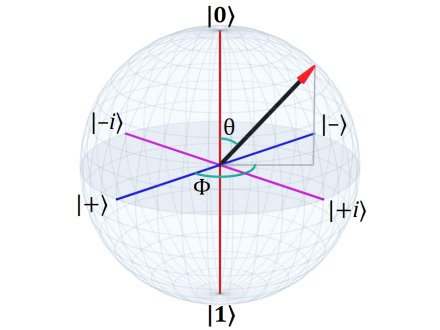
\includegraphics[scale=0.6]{images/bloch-hdr-440.png}
    \caption{Rappresentazione degli autovettori delle matrici di Pauli sulla sfera di Bloch. Il punto indicato dalla freccia rossa indica un generico qubit.}
    \label{fig:BlochSphere2}
\end{figure}

\noindent Come detto in precedenza, le 3 matrici di Pauli parametrizzano lo spin e i 3 assi della sfera di Bloch possono essere associati allo spin. Considerando lo stato generico $\ket{\psi}$ della \eqref{generic qubit}, possiamo definire lo spin lungo una direzione generica $\vec{\sigma} \cdot \vec{n}$ dove $\vec n = (\cos\phi\sin\theta, \sin\phi\sin\theta, \cos\theta)$:

\begin{equation*}
    \vec{\sigma} \cdot \vec n = \cos\phi\sin\theta \, \sigma_1 + \sin \phi \sin \theta \, \sigma_2 + \cos \theta \, \sigma_3 \, ;
\end{equation*}
così facendo è un semplice esercizio di QM dimostrare che $\ket{\psi}$ è autostato di $\vec{\sigma} \cdot \vec n$ con autovalore 1, ossia $\vec{\sigma} \cdot \vec n \ket{\psi} = \ket{\psi}$. Questo significa che dato uno stato sulla sfera di Bloch, allora esso è anche autostato di spin nella direzione individuata da tale qubit: infatti l'idea fisica alla base della sfera di Bloch è che la direzione arbitraria scelta non è altro che la direzione della quantizzazione dello spin. 

\section{Misurazioni}

\begin{itemize}
    \item \textbf{III Postulato} (\textbf{Regola di Born}):
    \begin{enumerate}
        \item \textbf{Misurazione}: sia $\hat{A}$ un osservabile con autostati $\ket{n}$, ossia $\hat{A} \ket{n} = a_n \ket{n}$. Prendiamo per semplicità $a_n \neq a_m \ \forall \, n \neq m$ (osservabile con autovalori distinti). Consideriamo uno stato generico espanso sugli autostati precedenti: $\ket \psi = \sum_n \alpha_n \ket n$. Allora una misura dell'osservabile $\hat{A}$ produce il valore $a_n$ con probabilità data da $\abs{\alpha_n}^2$ (assumendo lo stato correttamente normalizzato).
        
        \item \textbf{Collasso dello stato}: cosa succede allo stato del sistema dopo la misurazione? Istantaneamente lo stato $\ket \psi$ collassa sull'autostato associato all'autovalore risultante dalla misura. Ad esempio se misurando otteniamo $a_n$ allora $\ket{\psi} \rightarrow \ket{n}$. Effettuando delle misure successive sullo stato si ottiene sempre $\ket{n}$ con probabilità esattamente uguale a 1.  
    \end{enumerate}
\end{itemize}

\begin{esempio}
    Consideriamo per esempio il generico qubit in \eqref{generic qubit} e immaginiamo di voler effettuare delle misurazioni in differenti basi. Supponiamo di voler misurare lo spin lungo $z$ (base $\lbrace \ket{0}, \ket{1} \rbrace$ di $\sigma_3$) e lungo $x$ (base $\lbrace \ket{+}, \ket{-} \rbrace$ di $\sigma_1$). Essendo il qubit già decomposto sulla base computazionale, una misurazione lungo $z$ produrrà
    
    \begin{equation*}
        P(\ket{0}) = \abs{\cos \! \left( \frac{\theta}{2} \right)}^2 \, , \qquad P(\ket{1}) = \abs{\sin \! \left( \frac{\theta}{2} \right)}^2 \, .
    \end{equation*}
    
    \noindent Per capire il risultato della misurazione lungo $x$, invece, dobbiamo espandere $\ket{\psi}$ sulla base $\lbrace \ket{+}, \ket{-} \rbrace$: usando le \eqref{basi_di_sigma_12} per esprimere $\lbrace \ket{0}, \ket{1} \rbrace$ in termini di $\lbrace \ket{+}, \ket{-} \rbrace$ ricaviamo
    
    \begin{equation*}
        P(\ket{+}) = \frac{1}{2} \abs{\cos \! \left( \frac{\theta}{2} \right) + e^{i \phi} \sin \! \left( \frac{\theta}{2} \right)}^2 \, , \qquad P(\ket{-}) = \frac{1}{2} \abs{\cos \! \left( \frac{\theta}{2} \right) - e^{i \phi} \sin \! \left( \frac{\theta}{2} \right)}^2 \, .
    \end{equation*}
    
    \noindent Si noti come in entrambe le situazioni la probabilità risulta correttamente normalizzata: $P(\ket{0}) + P(\ket{1}) = P(\ket{+}) + P(\ket{-}) = 1$. 
\end{esempio}

\begin{esempio}
    Consideriamo lo stato $\ket{+}$ delle \eqref{basi_di_sigma_12}. Qual è l'interpretazione fisica di tale stato? Supponiamo che rappresenti lo spin di una particella: quando lo spin si trova in $\ket{+}$ allora sappiamo con certezza che punta lungo la direzione $x$, ossia $P(\ket{+}) = 1$. Al contrario, per una misurazione lungo $z$ sappiamo che $P(\ket{0}) = 1/2$ e $P(\ket{1}) = 1/2$: abbiamo la certezza del risultato lungo l'asse $x$, ma lungo l'asse $z$ si ha totale incertezza. Questo fenomeno è dovuto alla non commutatività degli operatori di spin nelle 3 direzioni:
    
    \begin{equation*}
        \comm{\hat{S}_i}{\hat{S}_j} = i \hbar \varepsilon_{ijk} \hat{S}_k \, .
    \end{equation*}
    
    \noindent Se consideriamo infatti il sistema preparato in $\ket{+}$ e supponiamo di effettuare una misura lungo $z$ ottenendo $\ket{0}$ allora lo stato collasserà in $\ket{0}$ e, d'ora in avanti, qualsiasi misurazione lungo $z$ produrrà sempre $\ket{0}$ con $P(\ket{0}) = 1$. Nonostante ciò, il fatto che $\hat{S}_z$ non commuti con $\hat{S}_x$ fa sì che una misura successiva lungo $x$ "rigeneri" dell'incertezza: $P(\ket{+}) = 1/2$ e $P(\ket{-}) = 1/2$ (si veda $\ket{0}$ espresso in termini di $\lbrace \ket{+}, \ket{-} \rbrace$ dalle \eqref{basi_di_sigma_12}). 
\end{esempio}

\noindent Discutiamo la generalizzazione del III postulato nel caso in cui alcuni autovalori associati ad autostati differenti siano uguali, cioè siamo in presenza di \textbf{degenerazione}. Per esempio supponiamo il caso $N = \dim \mathcal{H} = 6$: 

\begin{equation*}
    \ket \psi = \alpha_1 \ket 1 + \alpha_2 \ket 2 + \alpha_3 \ket 3 + \alpha_4 \ket 4 + \alpha_5 \ket 5 + \alpha_6 \ket 6 \, , 
\end{equation*}

\noindent dove supponiamo la degenerazione su $a_1 = a_2$ e $a_4 = a_5 = a_6$. Introduciamo gli operatori $\hat{P}_{a_i}$ che considerano solamente la parte di $\ket{\psi}$ corrispondente all'autospazio associato ad $a_i$:

\begin{equation*}
    \ket \psi = \underbrace{\alpha_1 \ket 1 + \alpha_2 \ket 2 }_{\hat P_{a_1} \ket \psi} + \underbrace{\alpha_3 \ket 3}_{\hat P_{a_3} \ket \psi} + \underbrace{\alpha_4 \ket 4 + \alpha_5 \ket 5 + \alpha_6 \ket 6}_{\hat P_{a_4 \ket \psi}} \, ;
\end{equation*}

\noindent tali operatori prendono il nome di \textbf{proiettori} e soddisfano le proprietà seguenti:  
\begin{enumerate}
    \item $\hat P_{a_i}^\dagger = \hat P_{a_i}$;
    \item $\hat P_{a_i}^2 = \hat P_{a_i}$;
    \item $\sum_i \hat P_{a_i} = \mathbb{I}$. 
\end{enumerate}

\noindent I proiettori sono utili per scrivere la \textbf{regola di Born} (III postulato) nel caso generale: dato uno stato $\ket{\psi}$ con degenerazione sugli autovalori $a_i$, la probabilità di ottenere il risultato $a_n$ è

\begin{equation*}
    P(a_n) = \norm{\hat{P}_{a_n} \ket{\psi}}^2 \, ;
\end{equation*}

\noindent dopo la misura, la funzione d'onda collassa nel seguente stato normalizzato:

\begin{equation*}
    \ket{\psi} \rightarrow \frac{\hat{P}_{a_n} \ket{\psi}}{\norm{\hat{P}_{a_n} \ket{\psi}}} \, .
\end{equation*}

\noindent Ad esempio, nel caso dello stato sopra scritto, la probabilità di ottenere $a_1 = a_2$ non è altro che 

\begin{equation*}
    P(a_1) = \norm{\hat{P}_{a_1} \ket{\psi}}^2 = \norm{\alpha_1 \ket{1} + \alpha_2 \ket{2}}^2 = \abs{\alpha_1}^2 + \abs{\alpha_2}^2 \, ,
\end{equation*}

\noindent e lo stato collassa in

\begin{equation*}
    \ket{\psi} \rightarrow \frac{\alpha_1 \ket{1} + \alpha_2 \ket{2}}{\sqrt{\abs{\alpha_1}^2 + \abs{\alpha_2}^2}} \, ;
\end{equation*}

\noindent si noti che si ha ancora incertezza su in quale stato si trovi $\ket{\psi}$, ma con un esperimento successivo \textbf{diverso} siamo in grado di risolvere la degenerazione e ottenere $\ket{1}$ o $\ket{2}$. 

\section{Evoluzione temporale}
Il postulato successivo riguarda l'evoluzione temporale degli stati:

\begin{itemize}
    \item \textbf{IV Postulato} (\textbf{Evoluzione temporale}): L'evoluzione temporale di uno stato generico $\ket{\psi(0)}$ è descritta dall'equazione di Schrödinger:
    
    \begin{equation*}
        i \hbar \dv{t} \ket{\psi(t)} = \hat H \ket{\psi(t)} \, ,
    \end{equation*}
    
    \noindent dove $\hat{H}$ è l'operatore (hermitiano) \textbf{hamiltoniana} del sistema. L'equazione di Schrödinger conserva le probabilità: $\braket{\psi(t)} = \braket{\psi(0)} = 1$. 
\end{itemize}

\noindent Solitamente si risolve questa equazione introducendo l'\textbf{operatore di evoluzione temporale} $\hat{U}(t)$:

\begin{equation*}
    \ket{\psi(t)} = \hat{U}(t) \ket{\psi(0)} \, ;
\end{equation*}

\noindent quando l'hamiltoniana è indipendente dal tempo, $\hat{U}(t)$ diventa semplicemente

\begin{equation*}
    \hat{U} (t) = e^{-\frac{i}{\hbar} \hat H t} \, ;
\end{equation*}

\noindent se invece $\hat H = \hat H(t)$, è necessario distinguere i casi di hamiltoniane commutanti o non commutanti a tempi differenti.\\
\noindent Come detto sopra, l'evoluzione temporale preserva le probabilità e ciò è una diretta conseguenza del fatto che $\hat{U}(t)$ sia \textbf{unitario}: 
\begin{itemize}
    \item $\hat U \hat U^\dagger = \hat U^\dagger U = \mathbb{I} \quad \Rightarrow \quad \hat{U}^\dagger = \hat{U}^{-1}$.
    \item Il prodotto scalare è conservato: $\braket{\hat U\phi}{\hat U\psi} = \braket{\phi}{\hat U^\dagger \hat U\psi} = \braket{\phi}{\psi}$. 
\end{itemize}
\noindent Notiamo che $\hat{U}(t)$ per hamiltoniane indipendenti da $t$ è effettivamente unitario:

\begin{equation*}
    \hat U^\dagger \hat U = \left( e^{-\frac{i}{\hbar} \hat H t} \right)^\dagger e^{-\frac{i}{\hbar} \hat H t} = e^{\frac{i}{\hbar} \hat H t} e^{-\frac{i}{\hbar} \hat H t} = \mathbb{I} \, .
\end{equation*}

\section{Gate}\label{sec:gate}

\begin{definizione}[\textbf{Porte quantistiche}]
    L'analogo quantistico delle porte (o gate) logiche classiche sono le \textbf{porte quantistiche} (o \textbf{gate quantistici}). Un gate quantistico è un operatore unitario che cambia lo stato del sistema.
\end{definizione}

\noindent Notiamo che una delle principali differenze che rendono di difficile implementazione le porte quantistiche risiede nel fatto che non possiamo implementare direttamente le più semplici operazioni classiche come \texttt{AND}, \texttt{OR} o \texttt{XOR}. 

\begin{definizione}[\textbf{Circuito Quantistico}]
    Un \textbf{circuito quantistico} è un modello di computazione quantistica in cui una sequenza ordinata di gate quantistici è applicata ai qubit.
\end{definizione}

\noindent In un circuito classico l'uso dei gate logici è banale. Supponiamo di considerare un bit che si trova in 0 o 1: un gate costituisce l'implementazione di un agente esterno che cambia lo stato del bit. Si pensi ad esempio al gate \texttt{NOT} per il quale $a \rightarrow$ \texttt{NOT} $a$:
\begin{center}
    \begin{circuitikz}
        \draw
        (0,4.5) node[not port] (mynot) {}
        (mynot.in) node[left = .4cm, anchor=east] (a) {$0$}
        (mynot.out) node[right = .4cm,anchor=west] (b) {$1 \, ,$}
        (mynot.in) -- (a)
        (mynot.out) -- (b);
    \end{circuitikz}
    $\qquad$
    \begin{circuitikz}
        \draw
        (0,4.5) node[not port] (mynot) {}
        (mynot.in) node[left = .4cm, anchor=east] (a) {$1$}
        (mynot.out) node[right = .4cm,anchor=west] (b) {$0 \, ,$}
        (mynot.in) -- (a)
        (mynot.out) -- (b);
    \end{circuitikz}
\end{center}

\noindent Nel caso invece di un qubit, i circuiti funzionano diversamente perché le porte agiscono su sistemi a due livelli. Immaginiamo che a causa di un agente esterno il qubit $\ket{\psi}$ subisca un evoluzione temporale $\hat{U}$: rappresentiamo questo fatto mediante il circuito seguente
\begin{center}
    \mbox{
        \Qcircuit @C=2em @R=2em {
            \lstick{\ket{\psi}} & \gate{\hat{U}} & \rstick{\hat{U} \ket{\psi} \, ,} \qw \\
        }
    }
\end{center}

\noindent Si ricordi che $\hat{U}$ è sempre un operatore unitario: ad esempio per un'hamiltoniana indipendente dal tempo si ha semplicemente $\hat{U}(t) = e^{-\frac{i}{\hbar}\hat H t}$. \\
\noindent Consideriamo le matrici di Pauli: sappiamo che sono hermitiane ($\sigma^\dagger_i = \sigma_i$) e che soddisfano la proprietà $\sigma_i^2 = \mathbb{I}$, ma questo significa che sono anche matrici unitarie. Questo fatto ci permette di costruire\footnote{Un tale sistema in natura è abbastanza semplice da implementare poiché, essendo $\hat{H} = \vec{\sigma} \cdot \vec B$ l'accoppiamento tra spin e campo magnetico, è facile costruire una tale evoluzione temporale.} dei gate in cui $\hat{U} = \hat{\sigma}_i$.  Ad esempio è possibile implementare dei gate come $\mathbb{I}$, $\sigma_1 \equiv X$, $\sigma_2 \equiv Y$ e $\sigma_3 \equiv Z$. Ricordando che $\sigma_i \sigma_j = i \varepsilon_{ijk} \sigma_k$ per $i \neq j$, notiamo che $XZ = - i Y$ e inoltre anche la matrice $-iY$ è unitaria. Per tale ragione molto spesso, al posto di considerare i gate $\lbrace \mathbb{I}, X, Y, Z \rbrace$ si sceglie la base $\lbrace \mathbb{I}, X, Z, XZ \rbrace$: questo significa che possiamo implementare i gate seguenti
\begin{center}
    \mbox{
        \Qcircuit @C=2em @R=2em {
            & \gate{X} & \qw \\
        }
    } 
    , \ \ \ \ 
    \mbox{
        \Qcircuit @C=2em @R=2em {
            & \gate{Z} & \qw \\
        }
    }
    , \ \ \ \ 
    \mbox{
        \Qcircuit @C=2em @R=2em {
            & \gate{XZ} & \qw \\
        }
    }
    ,
\end{center}

\noindent Consideriamo l'\texttt{X-gate}: dalle \eqref{Pauli_matrices} è evidente che $X$ rappresenta una sorta di "quantum" \texttt{NOT} perché inverte semplicemente lo stato della base computazionale:
\begin{center}
    \mbox{
        \Qcircuit @C=2em @R=2em {
            \lstick{\ket{0}} & \gate{X} & \rstick{\ket{1} \, ,} \qw \\
        }
    } 
    \\
    \mbox{
        \Qcircuit @C=2em @R=2em {
            \lstick{\ket{1}} & \gate{X} & \rstick{\ket{0} \, ,} \qw \\
        }
    }
\end{center}

\noindent Consideriamo ora lo \texttt{Z-gate}: gli stati della base computazionale sono autovettori con autovalori 1 e $-1$ di $\sigma_3$, quindi questo gate inverte semplicemente il segno
\begin{center}
    \mbox{
        \Qcircuit @C=2em @R=2em {
            \lstick{\ket{0}} & \gate{Z} & \rstick{\ket{0} \, ,} \qw \\
        }
    } 
    \\
    \mbox{
        \Qcircuit @C=2em @R=2em {
            \lstick{\ket{1}} & \gate{Z} & \rstick{-\ket{1} \, ,} \qw \\
        }
    }
\end{center}
L'azione dello \texttt{Z-gate} su un generico qubit risulterà quindi in
\begin{center}
    \mbox{
        \Qcircuit @C=2em @R=2em {
            \lstick{a \ket{0} + b \ket{1}} & \gate{Z} & \rstick{a \ket{0} - b \ket{1} \, ,} \qw \\
        }
    } 
\end{center}
e questo significa che $Z$ aggiunge semplicemente una fase $e^{i \pi} = -1$ allo stato. Ricapitolando: l'\texttt{X-gate} implementa un'interferenza dall'esterno che inverte lo stato (ad esempio cambia segno dello spin lungo $z$) e lo \texttt{Z-gate} implementa l'introduzione di una fase. \\
\noindent Una matrice particolarmente importante per i nostri scopi è 
\begin{equation}\label{Hadamard_matrix}
    H = \frac{1}{\sqrt{2}} 
    \begin{pmatrix}
        1 & 1 \\ 1 & -1 
    \end{pmatrix} \, , 
\end{equation}
chiamata \textbf{matrice di Hadamard}. Notiamo che è unitaria in quanto $H^\dagger H = \mathbb{I}$. Essa può essere implementata nel cosiddetto \texttt{H-gate} o \textbf{gate di Hadamard}: si tratta di un gate particolarmente importante (lo useremo largamente durante tutto il corso) in quanto permette di cambiare base $\lbrace \ket{0}, \ket{1} \rbrace \leftrightarrow \lbrace \ket{+}, \ket{-} \rbrace$ 

\begin{center}
    \mbox{
        \Qcircuit @C=2em @R=2em {
            \lstick{\ket{0}} & \gate{H} & \rstick{\ket{+} \, ,} \qw \\
        }
        \ \ \ \ \ \ \ \ \ \ \ \ \ \ \ \ \ \ \ \ 
        \Qcircuit @C=2em @R=2em {
            \lstick{\ket{+}} & \gate{H} & \rstick{\ket{0}\, ,} \qw \\
        }
    }
    \\
    \mbox{
        \Qcircuit @C=2em @R=2em {
            \lstick{\ket{1}} & \gate{H} & \rstick{\ket{-} \, ,} \qw \\
        } 
        \ \ \ \ \ \ \ \ \ \ \ \ \ \ \ \ \ \ \ \ 
        \Qcircuit @C=2em @R=2em {
            \lstick{\ket{-}} & \gate{H} & \rstick{\ket{1} \, ,} \qw \\
        }
    }
\end{center}

\noindent Possiamo introdurre anche le matrici seguenti (ci serviranno più avanti)

\begin{equation}\label{S_T_matrices}
    S \equiv \sqrt{Z} =
\begin{pmatrix}
    1 & 0 \\ 0 & i
\end{pmatrix} \, , \qquad 
T \equiv \sqrt{S} =
\begin{pmatrix}
    1 & 0 \\ 0 & e^{i \frac{\pi}{4}}
\end{pmatrix} \, ,
\end{equation}

\noindent Le matrici introdotte in precedenza costituiscono gli oggetti base con cui andremo a implementare diversi gate e circuiti durante tutto il corso. Per costruire il gate più generale possiamo esponenziare scrivendo $U = e^{-\frac{i}{\hbar} H t}$ dove $H = a \mathbb{I} + b_i \sigma_i$ e $a, b_i \in \mathbb{R}$ con $i = 1,2,3$. Esiste una particolare classe di operatori che utilizzeremo molto dati da
\begin{equation*}
    R_{\vec{n}}(\lambda) = e^{-i \frac{\lambda}{2} (\vec n \cdot \vec \sigma)} \, ;
\end{equation*}
si tratta di un caso particolare dell'esponenziazione precedente in cui $a = 0$ e i coefficienti $b_i$ sono scelti lungo un particolare versore $\vec n$. Questo operatore unitario implementa una rotazione di angolo $\lambda$ attorno alla direzione individuata da $\vec n$:

\begin{equation}\label{rotation_n_lambda}
    R_{\vec{n}}(\lambda) = e^{-i \frac{\lambda}{2} (\vec n \cdot \vec \sigma)} = \cos \! \left( \frac{\lambda}{2} \right) \mathbb{I} - i \sin \! \left( \frac{\lambda}{2} \right) \vec \sigma \cdot \vec n \, ;
\end{equation}
(si espanda il LHS con la serie di Taylor dell'esponenziale e si usi $(\vec \sigma \cdot \vec n)^2 = \mathbb{I}$ per dimostrare l'uguaglianza con il RHS). È possibile dimostrare, inoltre, che qualsiasi matrice unitaria $2 \times 2$ può essere scritta nella forma seguente
\begin{equation}\label{general_2by2_matrix}
    U = e^{i \alpha}
    \begin{pmatrix}
        e^{-i \frac{\beta}{2}} & 0 \\ 0 & e^{i \frac{\beta}{2}}
    \end{pmatrix}
    \begin{pmatrix}
        \cos \frac{\gamma}{2} & - \sin \frac{\gamma}{2} \\ \sin  \frac{\gamma}{2} & \cos \frac{\gamma}{2}
    \end{pmatrix}
    \begin{pmatrix}
        e^{-i \frac{\delta}{2}} & 0 \\ 0 & e^{i \frac{\delta}{2}}
    \end{pmatrix}
    = e^{i \alpha} R_z(\beta) R_x(\gamma) R_z(\delta) \, ; 
\end{equation}
perciò il più generale operatore unitario presenta 4 parametri reali $\alpha, \beta, \gamma, \delta \in \mathbb{R}$ e può implementare un possibile gate in un computer quantistico. Appare subito evidente come la scelta di 4 possibili parametri reali (quindi continui) consenta di realizzare un numero nettamente maggiore di gate logici quantistici rispetto al caso dei gate logici classici. 
    \vspace{1cm}
\newline
\lecture{3}{14/10/2021}
\vspace{0.5cm}
\noindent Abbiamo visto come sia possibile calcolare il valore di aspettazione di $\expval{A}$ a partire dalle funzioni d'onda. Vogliamo vedere come sia possibile sfruttare la matrice densità per ottenere il medesimo risultato. Cominciamo considerando il generico insieme di stati $\{p_i, \ket{\psi_i}\}$ e la matrice densità corrispondente $\hat \rho=\sum_i p_i\op{\psi_i}{\psi_i}$. Per il singolo stato $\ket{\psi_i}$ avevamo visto che
\begin{equation*}
    \begin{aligned}
        \expval{A}_{\psi_i} &= \sum_k p_k a_k \\
                            &= \sum_k \ip{\psi_i}{a_k}\ip{a_k}{\psi_i}a_k \\
                            &= \bra{\psi_i}\sum_k a_k \ket{a_k}\ip{a_k}{\psi_i} \\
                            &= \expval{A}{\psi_i}
    \end{aligned}
\end{equation*}
Tuttavia, nel caso della matrice densità, abbiamo un insieme di funzioni d'onda, per cui
\begin{equation*}
    \begin{aligned}
        \expval{A} &= \sum_i p_i \expval{\hat A}{\psi_i} \\
                   &= \sum_i p_i \Tr \left(\hat A\op{\psi_i}{\psi_i}\right) \\
                   &= \Tr \left(A\sum_i p_i \op{\psi_i}{\psi_i}\right) \\
                   &= \Tr\left(\hat A\rho\right) \, .
    \end{aligned}
\end{equation*}

\subsection*{Equazione di von-Neumann - Liouville}
Per il \textbf{IV Postulato}, riguardante l'evoluzione temporale, la matrice densità evolve come $\hat U \hat \rho \hat U^\dagger$, ci chiediamo se sia possibile realizzare un'equazione analoga a quella di Schrödinger per la matrice densità. La risposta è affermativa, infatti
\begin{equation*}
    \begin{aligned}
        \derivative{\hat \rho}{t} &= \sum_i p_i\left(\derivative{\ket{\psi_i}}{t}\bra{\psi_i}+\ket{\psi_i}\derivative{\bra{\psi_i}}{t}\right) \\
                                  &= \sum_i \frac{p_i}{i\hbar}\left(\hat H \op{\psi_i}{\psi_i}-\op{\psi_i}{\psi_i}\hat H\right) \\
                                  &= \frac{1}{i\hbar}\comm{\hat H}{\hat \rho}
    \end{aligned}
\end{equation*}

\noindent Consideriamo ora un paio di esempi per assodare i concetti finora trattati
\begin{esempio}
    Consideriamo un qubit nella base computazionale $\{\ket 0, \ket 1\}$ oppure possiamo pensare di prendere la base
    \begin{equation*}
        \ket a = \frac{\ket 0 +\ket 1}{\sqrt 2} \,
    \end{equation*}
    \begin{equation*}
        \ket b = \frac{\ket 0 -\ket 1}{\sqrt 2} \, ;
    \end{equation*}
    entrambe le basi sono degli stati puri.\\
    Consideriamo lo stato $\ket a$ e costruiamo la matrice densità per la base computazionale
    \begin{equation*}
        \hat \rho = \frac 12 \op{0}{0} + \frac 12 \op{1}{1} \, ,
    \end{equation*}
    come possiamo notare, gli stati hanno la medesima probabilità. Ora possiamo fare una \textbf{projective measurament} definendo i proiettori:
    \begin{itemize}
        \item $\hat P_0=\op{0}{0}$;
        \item $\hat P_1=\op{1}{1}$;
        \item $\hat P_a=\op{a}{a}$.
    \end{itemize}
    Andiamo a misurare le probabilità di misurare $\ket 0$ e $\ket 1$ sullo stato $\ket a$:
    \begin{equation*}
        p(\ket 0)=\mel{a}{\hat P_0}{a}=\frac 12 \quad \, , \quad p(\ket 1)=\mel{a}{\hat P_1}{a}=\frac 12 \, .
    \end{equation*}
    Cosa succede se consideriamo $\rho$?
    \begin{equation*}
        p(\ket 0)=\mel{0}{\hat \rho}{0}=\frac 12 \quad \, , \quad p(\ket 1)=\mel{1}{\hat \rho}{1}=\frac 12 \, .
    \end{equation*}
    Come possiamo notare otteniamo in entrambi i casi la medesima probabilità, se invece andassimo a misurare $\ket a$?
    \begin{equation*}
        \begin{aligned}
            p(\ket a) &= \mel{a}{\hat P_a}{a} \\
                      &= \ip{a}{a}\ip{a}{a} \\
                      &= 1 \, .
        \end{aligned}
    \end{equation*}
    Per quanto riguarda la matrice densità
    \begin{equation*}
        \begin{aligned}
            p(\ket a) &= \mel{a}{\hat \rho}{a} \\
                      &= \Tr \left(\hat \rho \op{a}{a}\right) \\
                      &= \frac 12 \, .
        \end{aligned}
    \end{equation*}
    In questo caso, misurare in un altra base ci dà due risultati differenti.
\end{esempio}
\noindent Questo esempio in realtà lo possiamo incontrare, dal punto di vista pratico, se ci addentriamo nello studio dello spin di un elettrone in un atomo (esperimento di Stern-Gerlach) oppure nella trattazione della polarizzazione di un fotone.

\noindent In generale noi possiamo scrivere la matrice densità in una base e poi riscriverla in un secondo momento in un'altra base
\begin{equation*}
    \hat \rho = \sum_k \omega_k \op{\psi_k}{\psi_k} \, ,
\end{equation*}
dove 
\begin{equation*}
    \{\omega_k, \ket{\psi_k}\} \quad \text{e} \quad \ket{\psi_k}=\sum_j a_j^k \ket{a_j} \, .
\end{equation*}
Nella nuova base, la matrice densità sarà
\begin{equation*}
    \begin{aligned}
        \hat \rho &= \sum_k {\omega_k}\left(\sum_j a_j^k \ket{a_j}\right)\left(\sum_i a_i^{*k}\bra{a_i}\right) \\
             &= \sum_{k,j,i} \omega_k a_j^ka_i^{*k}\op{a_j}{a_i}
    \end{aligned}
\end{equation*}
per cui gli elementi di matrice saranno
\begin{equation*}
    \begin{aligned}
        \rho_{mn} &= \mel{a_m}{\hat \rho}{a_n} \\
                       &= \sum_k \omega_k a_m^ka_n^{*k}
    \end{aligned}
\end{equation*}
e gli elementi sulla diagonale
\begin{equation*}
    \rho_{nn}=\sum_k\omega_k \abs{a_n^k}^2
\end{equation*}

\subsection{POVM: Misura a valori operatoriali positivi}
Molti tipi di misurazione, come ad esempio la rivelazione della posizione di un fotone, non possono essere visti come proiezioni perché lo stato dopo la misura viene distrutto. Nel caso considerato, quando misuriamo il fotone esso viene assorbito dal rivelatore e non esiste più. A differenza delle misure proiettive non posso effettuare un'ulteriore misura sullo stesso stato. La proiezione non permette inoltre di distinguere in maniera esatta due stati non ortogonali. Ad esempio presi due stati $\ket \psi$ e $\ket \phi$, se sono tra loro ortogonali sarà facile distinguerli con i proiettori, ma se non sono ortogonali non possiamo distinguerli e gli unici risultati che possiamo dare sono:
\begin{itemize}
    \item È nello stato $\ket \psi$;
    \item È nello stato $\ket \phi$;
    \item O in qualcos'altro.
\end{itemize}
Una misura a valori operatoriali positivi (POVM) è una misura i cui valori sono operatori semi-definiti positivi su uno spazio di Hilbert che non richiedono ortogonalità, cioè non soddisfano la terza proprietà che abbiamo visto quando abbiamo introdotto i proiettori: $\hat P_i \hat P_j = \hat P_i\delta_{ij}$. La POVM può essere utile per classificare uno stato con 3 possibili identificazioni (come $\ket \psi$, $\ket \phi$ o "non so") dove invece una misura proiettiva è inutile.

\subsection{Cambi di base: stati puri e miscele}

\noindent Supponiamo di avere una matrice densità $\hat \rho=\sum_i p_i \op{\psi_i}{\psi_i}$ e un'osservabile $\hat A$ ($\ket {a_k}$, $a_k$). Vogliamo valutare il valore di aspettazione di questa osservabile:
\begin{equation*}
    \begin{aligned}
        \expval{A} &= \Tr\left(\hat\rho \hat A\right) \\
                   &= \Tr\left(\sum_{ijk} \rho_{ij}\op{a_i}{a_j}a_k\op{a_k}{a_k}\right) \\
                   &= \sum_{ik}\rho_{ik}a_k\Tr\left(\op{a_i}{a_k}\right) \\
                   &= \sum_{ik}\rho_{ik}a_k\ip{a_k}{a_i} \\
                   &= \sum_k\rho_{kk}a_k
    \end{aligned}
\end{equation*}
Quindi, solo i $\rho_{kk}=\mel{a_k}{\rho}{a_k}$ sono necessari per calcolare il valore di aspettazione e gli elementi off-diagonal nella nostra rappresentazione sono apparentemente inutili. Tuttavia, gli elementi off-diagonal spesso ci dicono se la matrice corrisponde a uno stato puro o meno. Se abbiamo una matrice di densità non diagonale in una base di un'osservabile, anche se il valore di aspettazione dell'osservabile stessa è dato solo dagli elementi diagonali, se gli elementi off-diagonal sono diversi da zero allora lo stato può essere puro, poiché la matrice diagonalizzata può avere tutte le voci uguali a $0$, tranne una uguale a $1$. Questi elementi fuori diagonale sono chiamati coerenza della matrice densità. Per esempio, consideriamo la seguente matrice $2\times 2$
\begin{equation*}
    \begin{pmatrix}
        a & c \\
        c^* & b
    \end{pmatrix}
\end{equation*}
I coefficienti $c$ e $c^*$ prendono il nome di \textbf{coerenze}, questo perché:
\begin{itemize}
    \item Se $c=c^*=0$, allora abbiamo una miscela di stati;
    \item Se $c,c^*\neq 0$, allora possiamo avere uno stato puro, in quanto la matrice può essere diagonalizzata nella forma
        \begin{equation*}
            \begin{pmatrix}
                1 & 0 \\
                0 & 0
            \end{pmatrix}
        \end{equation*}
\end{itemize}
Osserviamo che, generalmente, $c$ e $c^*$ seguono una legge di decadimento, per cui scalano come $e^{-t/T_1}$, il che significa che lo stato sta perdendo la sua purezza al passare del tempo. Questo è uno dei problemi più importanti quando si lavora con dei sistemi come i qubit, in quanto ne limita il suo utilizzo.
\end{document}
